
\phantomsection
\numberedsection{RF8 Gestión de Exportación}

\paragraph{Descripción:}
Permite a los usuarios exportar productos seleccionados desde el sistema Mini PIM a Amazon, con atributos obligatorios y opcionales configurables por el usuario.

\paragraph{Precondición:}
\begin{itemize}
    \item El usuario ha iniciado sesión en Mini PIM.
    \item Existen productos en el sistema con los atributos obligatorios necesarios.
\end{itemize}

\paragraph{Postcondición:}
\begin{itemize}
    \item \textbf{Caso de éxito:} Los productos seleccionados son exportados exitosamente al formato CSV requerido por Amazon y están listos para su carga.
    \item \textbf{Caso de error:} El sistema notifica al usuario cualquier error o dato faltante, permitiendo realizar las correcciones necesarias.
\end{itemize}

\paragraph{Prioridad:}
Alta
\paragraph{Autor:}
Diego Sicre.
\paragraph{Escenario Principal:}
\begin{enumerate}
    \item El usuario accede a la sección "Productos".
    \item El sistema muestra un listado de productos con los siguientes atributos:
    \begin{itemize}
        \item Thumbnail
        \item SKU
        \item Nombre
        \item Hasta tres atributos de usuario
    \end{itemize}
    \item El usuario puede filtrar los productos:
    \begin{itemize}
        \item Por categoría ingresándola en el desplegable al lado del calendario.
        \item Por fecha seleccionando un día en el calendario, con lo que el sistema mostrará todos los productos modificados desde dicha fecha hasta la actualidad.
    \end{itemize}  
    \item El usuario selecciona uno o más productos para exportar.
    \item El usuario hace click en el botón generar CSV.
    \item El sistema despliega un formulario para la configuración de mapeo de atributos general a todos los productos en el CSV, incluyendo:
    \begin{itemize}
        \item SKU: Se selecciona el SKU, para mapear en la exportación el SKU de cada producto en el sistema.
        \item Título: Se selecciona el Label del producto.
        \item Fulfilled by:  Nombre de la cuenta.
        \item Amazon\_SKU: Se permite al usuario seleccionar entre SKU/GTIN.
        \item Precio:  Se permite al usuario elegir un atributo de usuario como precio del producto.
        \item Offer Price: Booleano onfigurable como TRUE/FALSE/RANDOM general a todos los productos, indicando si el precio es de oferta.
    \end{itemize}
    \item El usuario confirma la configuración del mapeo obligatorio y selecciona Continuar.
    \item A continuación el sistema permite al usuario seleccionar atributos adicionales de usuario, que se exportarán al CSV.
    \item Seleccionando las checkbox, el usuario puede añadir los atributos de usuario, que maperán el nombre del atributo al contenido del mismo para cada producto.
    \item El sistema genera un archivo exportable en formato CSV, listo para ser cargado en Amazon.
    \item El usuario descarga el archivo generado.
\end{enumerate}

\paragraph{Escenarios Alternativos:}
\begin{itemize}
    \item \textbf{4.a: No hay productos seleccionados.}
    \begin{itemize}
        \item El sistema notifica al usuario que debe seleccionar al menos un producto para exportar.
    \end{itemize}
    \item \textbf{5.a: El sistema detecta que falta algún atributo obligatorio.}
    \begin{itemize}
        \item El sistema notifica al usuario qué falta algún atributo por configurar y le permite corregirlo.
    \end{itemize}
    \item \textbf{6.a: El usuario cancela la exportación.}
    \begin{itemize}
        \item El sistema regresa al listado de productos sin realizar ningún cambio.
    \end{itemize}
    \item \textbf{7.a: El usuario no selecciona atributos adicionales de usuario.}
    \begin{itemize}
        \item El sistema genera el CSV únicamente con los atributos obligatorios configurados.
    \end{itemize}
    \item \textbf{8.a: El usuario no encuentra el producto al filtrar por categoría.}
    \begin{itemize}
        \item El sistema muestra un mensaje indicando que no existen productos con esa categoría.
    \end{itemize}
    \item \textbf{8.b: El usuario no encuentra el producto al filtrar por fecha.}
    \begin{itemize}
        \item El sistema muestra un mensaje indicando que no hay productos disponibles en el rango seleccionado.
    \end{itemize}
\end{itemize}


\paragraph{Casos de Prueba:}
\begin{itemize}
    \item \textbf{Escenario Principal}
    \begin{itemize}
        \item \textbf{Dado:} Que el usuario ha iniciado sesión en Mini PIM y hay productos en el sistema.
        \item \textbf{Cuando:} Filtra por categoría y/o fecha
        \item \textbf{Y:} y selecciona productos
        \item \textbf{Y:} configura correctamente los mapeos.
        \item \textbf{Entonces:} El sistema genera un archivo exportable válido en formato CSV.
    \end{itemize}
    \item \textbf{Escenario Alternativo 4.a}
    \begin{itemize}
        \item \textbf{Dado:} Que el usuario intenta exportar sin seleccionar productos.
        \item \textbf{Cuando:} Confirma la acción.
        \item \textbf{Entonces:} El sistema muestra un mensaje de error indicando que debe seleccionar al menos un producto.
    \end{itemize}
    \item \textbf{Escenario Alternativo 5.a}
    \begin{itemize}
        \item \textbf{Dado:} Que el usuario ha iniciado la configuración del mapeo.
        \item \textbf{Cuando:} Intenta confirmar con un atributo obligatorio faltante.
        \item \textbf{Entonces:} El sistema notifica al usuario y solicita completar los datos faltantes.
    \end{itemize}
    \item \textbf{Escenario Alternativo 7.a}
    \begin{itemize}
        \item \textbf{Dado:} Que el usuario omite seleccionar atributos adicionales de usuario.
        \item \textbf{Cuando:} Finaliza la configuración de atributos obligatorios y selecciona Continuar.
        \item \textbf{Entonces:} El sistema genera el CSV solo con los atributos obligatorios.
    \end{itemize}
    \item \textbf{Escenario Alternativo 8.a}
    \begin{itemize}
        \item \textbf{Dado:} Que el usuario intenta buscar productos con una categoría específica.
        \item \textbf{Cuando:} No hay productos asociados a la categoría seleccionada.
        \item \textbf{Entonces:} El sistema muestra un mensaje indicando que no existen productos con esa categoría.
    \end{itemize}
    \item \textbf{Escenario Alternativo 8.b}
    \begin{itemize}
        \item \textbf{Dado:} Que el usuario selecciona un rango de fechas en el calendario.
        \item \textbf{Cuando:} No hay productos disponibles en el rango especificado.
        \item \textbf{Entonces:} El sistema muestra un mensaje indicando que no hay productos disponibles en el rango seleccionado.
    \end{itemize}
\end{itemize}
\paragraph{Boceto:}
\begin{figure}[H]
    \includegraphics[width=1\linewidth]{mockups/RF8 filtrado y selección de productos.png}
    \caption{Pantalla principal de exportación y formulario de configuración de mapeo.}
\end{figure}


\numberedsubsection{Bocetos}
\begin{figure}[H]
    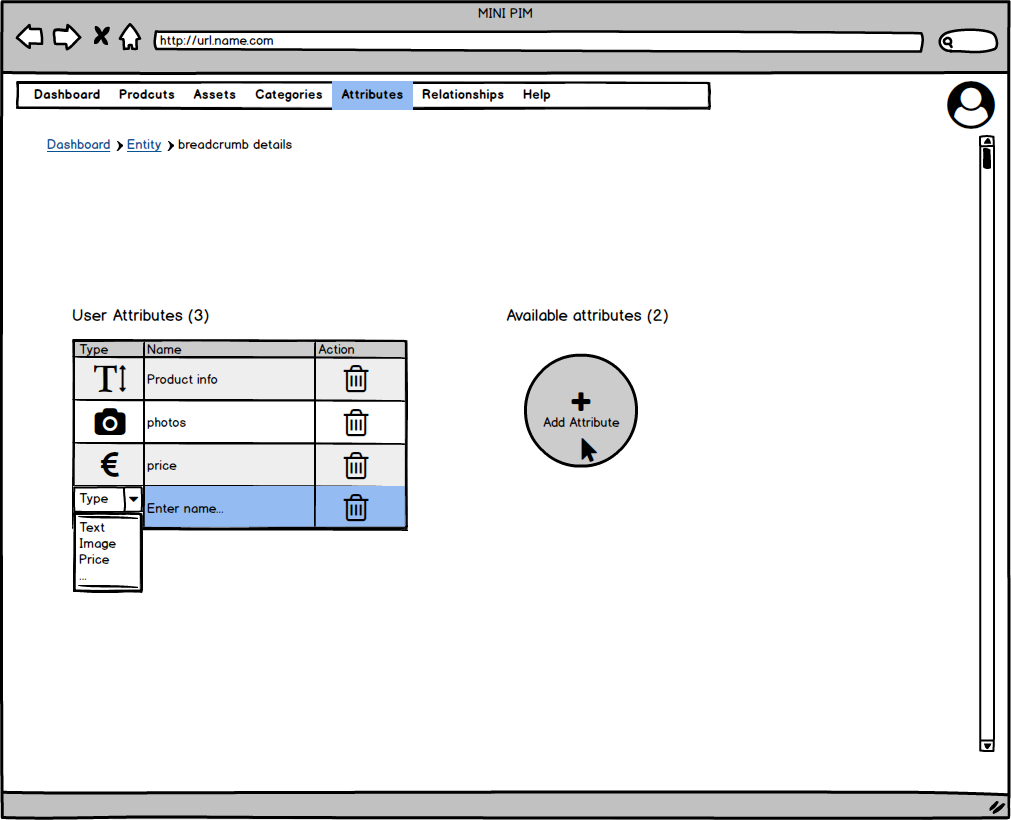
\includegraphics[width=1\linewidth]{mockups/RF6.1Crear_Atributo tras Clickar.png}
    \caption{Menú de creación tras clicar \enquote{Añadir atributo}}
   \end{figure}
\vspace{1.0cm}

\newpage %Inicia en una nueva página otro caso de uso